\documentclass[pdftex, a4paper]{scrartcl}
%\usepackage{ngerman}
\usepackage[utf8]{inputenc}
\usepackage[T1]{fontenc}
%\usepackage{array}
%\usepackage{subfiles}
\usepackage{url}
\usepackage[hidelinks]{hyperref}
\usepackage{parskip}
\setlength{\parskip}{1em}
\usepackage{xurl}
\usepackage[nottoc,notlot,notlof]{tocbibind}
\usepackage{setspace}
\linespread{1.5}
\usepackage[
top    = 2.75cm,
bottom = 2.50cm,
left   = 3.00cm,
right  = 2.50cm]{geometry}
\usepackage{etoolbox}
\AtBeginEnvironment{thebibliography}{\linespread{1}\selectfont}
\usepackage{endnotes}
\interfootnotelinepenalty=10000
\usepackage[acronym,toc,nonumberlist]{glossaries} 
\usepackage[titletoc]{appendix}
\usepackage{booktabs}
\usepackage{tabularx}
\usepackage{graphicx}
%\usepackage{textcomp}
\usepackage{lscape}
\usepackage{fancyhdr} 
\usepackage{multirow}
\usepackage{caption}
\usepackage{natbib}
\usepackage[table,xcdraw]{xcolor}
\usepackage{float}
%\usepackage{lineno}
\usepackage{longtable}
\makeglossaries

\newacronym{fao}{FAO}{Food and Agriculture Organization of the United Nations}
\newacronym{un}{UN}{United Nations}
\newacronym{api}{API}{Application Programming Interface}


\newglossaryentry{user} {
    name={User},
    plural={users},
    description={General description of a person who downloads and browses through the app without any direct intention
    of purchasing or offering a product}
}

\newglossaryentry{app} {
    name={App},
    description={It refers to the mobile application to be developed}
}
\newglossaryentry{stakeholder} {
    name={Stakeholder},
    plural={stakeholders},
    description={Describe all kind of potential person or entity that may have interest using the app}
}
\newglossaryentry{client} {
    name={Client},
    plural={clients},
    description={Since we have two major stakeholders that will use the app, the word client will
    specify the one that places an order in the app}
}
\newglossaryentry{provider} {
    name={Provider},
    plural={provider},
    description={The second major stakeholders are those who offer their products. They can begin
                restaurants, bakeries, pastries and similar}
}
\newglossaryentry{upload} {
    name={Upload},
    description={Will designate the act of pushing textual or visual content into the app. It will
                be mostly done by a provider}
}
\newglossaryentry{register} {
    name={Register},
    description={Describes the act of inputting name, e-mail, company name, product or any other kind of
    textual data used to identify a stakeholder or a product}
}
\newglossaryentry{activity diagram} {
    name={Activity Diagram},
    description={This kind of diagram shows the behavior of a system, it depicts in a graphical fashion 
    the logic of a single use case \cite{refinbook:Baresi2009}.}
}
\newglossaryentry{class diagram} {
    name={Class Diagram},
    description={This kind of diagram presents the structure of a system with its classes, attributes,
    methods and relationships\cite{refonline:IBMCD}}
}
\newglossaryentry{use case diagram} {
    name={Use Case Diagram},
    description={This kind of diagram presents the main requirements and functionality of a systems. It displays
    a simplified overview of core purpose of the application \cite{refart:YWRUS}}
}
\newglossaryentry{mobile payment gateway} {
    name={Mobile Payment Gateway},
    description={Those services works as an intermediary between customer, merchant and bank/credit card company. 
    Here a payment request is sent to the gateway and forwarded to the approval instances. The core functionality 
    of those gateways is the cryptography within the communication steps\cite{refonline:VPGI}}
}

\newglossaryentry{federated login} {
    name={Federated Login},
    description={Authentication method in which users use existing accounts to gain access to another domains or systems
    without the need of creating new credentials. The authenticity of a user is attested by service and granted to another 
    \cite{refonline:MRFL}}
}
\newglossaryentry{system response} {
    name={System Response},
    description={The output of a system after an input \cite{refonline:HWHE}.
    \cite{refonline:MRFL}}
}
\newglossaryentry{API} {
    name={Application Programming Interface - API},
    plural={APIs},
    description={Software intermediary that promotes the communication between different systems/applications/
    softwares\cite{refonline:MSAPI}}
}

% &as_qdr=y2 (find date)









\begin{document}
    \begin{titlepage}
    \vspace*{2mm}
    \begin{center}
        \Large
        \textbf{University for Applied Sciences}\\
        \textbf{Informatics Department}\\
        \textbf{Applied Informatics}\\
        \vspace{2cm}
        \textbf{To be defined}\\
        \vspace{2cm}
        \large
        Documentation for the Architecture of an Mobile Application for Preventing Food Waste\\
        \vspace{4cm}
        \begin {table}[ht]
            \centering
            \begin{tabular}{c}
                Bruno Macedo da Silva    \\ 
                676839                   \\
                inf3645@hs-worms.de      \\
            \end{tabular}
        \end {table}
        \vspace{2cm}
        \large
        \vspace{2cm}
         \begin {table}[ht]
             \centering
             \begin{tabular}{l l}
                Supervisor         & Prof. Dr. Volker Schwarzer \\
                Working Period:    & Summer Semester 2022 \\
                Due Date:          & 31.Juni 2022 \\
             \end{tabular}
         \end {table}
    \end{center}
    \normalsize
    \vfill
 


\end{titlepage}
    \tableofcontents
    %\newpage
    %\addcontentsline{toc}{section}{\listfigurename}
    %\listoffigures
    \newpage
    \clearpage
    \printglossary[type=acronym,title=Abbreviations,toctitle=Abbreviations]
    \clearpage
    \newpage
    \clearpage
    \printglossary[title=Glossary,toctitle=Glossary]
    \clearpage
    \section{Introduction and Goals}

According to the \acrfull{fao} in 2019, 931 millions tonne of food were wasted \cite{refart:FAOFW}. This has
environmental, but especially social consequences. In a world where approximately 9.9\% of the \cite{refart:AAHWH}
population suffers from hunger that waste percentage sounds paradoxal.

According to \acrfull{un} 5\% of the global food loss and waste comes from restaurants \cite{refart:UNSP}. 
The solution for this problem must be locally applied so its effects can be seen in a global structure. To do 
so we propose to develop a mobile application that connects restaurants, bakeries and or pastries to clients. The
former would offer their remaining products, which are still consumable, prior to the closing time, to a small price
and the latter would browser in the app to find which shops are offering products. 

We as ``Clean Up the World \textregistered'' are a rising StartUp whose main concerns is to find environmental solutions to
daily problems. Our portfolio includes projects about management of waste and optimization of household water 
usage. This product we want to develop targets small communities, like small cities or regions within a big city, 
to reduce the amount of wasted consumable food.

With our project we want to achieve the following goals:

\begin{itemize}
    \item Connect \glsplural{provider} with \glsplural{client}, so the former can offer products that the latter
    can purchase
    \item Collect statistical data about waste reduction within the \glsplural{provider}
    \item Promote reduction of food waste that still could be consumed
    \item Allow \glsplural{client} to have a different dining experience.
    \item Allow \glsplural{provider} to promote their products and gather new clients.
\end{itemize}

To make the easy to read we will use the pronouns ```he''' and ``his'' every time we refer to a single person.

\subsection{Design Purpose}

The main purpose of this architecture is creating an exploratory prototype of an \gls{app}. We aim to test it with potential 
\glsplural{stakeholder} and regions to analyze their general acceptance and wishes \cite{refbook:DSHC} and get a fast feedback. 

This prototype will also make it feasible to identify unknown needs an wishes of the potential \glsplural{stakeholder}, so we 
can eventually increase the scope of functionality. Exploring this domain will also provide us with information regarding 
the behavior of our target group when it comes to buying and serving food that would be wasted, but is still consumable.

\subsection{Requirement Overview} \label{Requirement_Overview}

The following functionalities describe the basic requirement for the \gls{app}:

\begin{table}[H]
    \setstretch{1.0}
    \begin{tabularx}{\textwidth}{llX}
    \toprule
    Id & Requirement & Description  \\
    \midrule
    F-1 & Register as \gls{client}. & A \gls{client} can register to the app with its e-mail.\\
    F-2 & Login & After registration \gls{client} can login into the app. \\
    F-3 & Purchase option & A registered \gls{client} can purchase an available offer (see F7).\\
    F-4 & Filter/search options & A \gls{client} can perform filter and search actions for products.\\
    F-5 & Register as \gls{provider} & A \gls{provider} can register his store and add logos and pictures.\\
    F-6 & Create offer & A registered \gls{provider} can publishes what products they are offering with price 
    and amount. \\
    F-7 & Upload offer & A registered \gls{provider} can add, edit or remove offers to his catalog.\\
    F-8 & Check orders & A registered \gls{provider} can check all existing orders targeting his/her shops.\\
    \bottomrule
    \end{tabularx}
\end{table}

\begin{table}[H]
    \setstretch{1.0}
    \begin{tabularx}{\textwidth}{lX}
    \toprule
    ID & Motivation \\
    \midrule
    F-1 & The entry door of the \gls{app}, where our \gls{client} get an overview of all available offers \\
    F-2 & In order to place purchases our client need to be registered. It will also provide 
    statistical information about consumer behavior \\
    F-3 & Since we are dealing with a business relationship we have on one side a client willing to pay
    and for a product and on the other side a provider willing to offer a product/service \\
    F-4 & Like any other online-shop it is important that our \gls{client} can browse through the available possibilities\\
    F-5 & In order to make a product available a \gls{provider} needs to register his/her shop. This information will
    also be used for statistical analyzes about providers, products and consumer behavior \\
    F-6 - F-7 & A registered \gls{provider} can make an offer available according to his/her daily planning. 
    For future development of this app, this will be helpful to identify tendencies regarding dates, periods 
    and availabilities. \\
    F-8 & Also registered \glsplural{provider} can get an overview about how often their products have been sold. This
    may open a different kind of business orientation. \\
    \bottomrule
    \end{tabularx}
\end{table}


The following \gls{use case diagram} displays an overview of the primary functionality of the app:

\begin{figure}[H]
    \centering
    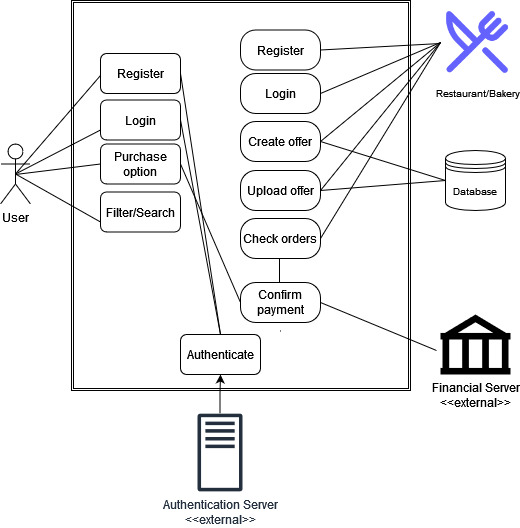
\includegraphics[width=0.5\textwidth]{assets/preliminary_functions.jpg}
    \caption{Preliminary functions}
    \label{fig:preliminary_use_case}
\end{figure}

\newpage
\subsection{Qualitiy Goals}

The key qualities of this app are described in the table below:

\begin{table}[H]
    \setstretch{1.0}
    \begin{tabularx}{\textwidth}{|c|c|X|}
        \toprule
        \multicolumn{1}{c}{Quality} & \multicolumn{1}{c}{Priority} & \multicolumn{1}{c}{Motivation} \\
        \midrule
        \textbf{Usability} & 1 & Since we are working with a prototype it is important the usage is easy as possible,
        to attract more \glsplural{user} and to gather information about consumer behaviour. \glsplural{client} and \glsplural{provider}
        should have a simple interface where they can quickly interact without any burdens. \\
        \textbf{Interoperability} & 2 & To reduce programming burdens and accelerate the delivery of a working product the
        registration and payment process will rely on third party providers. For that reason the developed features should
        work faultless in combination with the external \glsfirst{API} (i.g \gls{mobile payment gateway} and \gls{federated login}). \\
        \textbf{Performance} & 3 & Many mobile and web-apps lose potential \glsplural{user} because of the lack of performance. A 
        \gls{system response} that takes too long (more than 1 second \cite{refonline:AP16M}) may frustrate potential \glsplural{user} 
        and discourage them of using the application. \\
        \textbf{Security} & 4 & To guarantee a secure and easy payment process we will handle the \gls{API} of the 
        \gls{mobile payment gateway} within the development process. The possibility of outsourcing this service would cause
        a big damage to the first priority. \\
        \bottomrule
    \end{tabularx}
\end{table}

\newpage

\subsection{Stakeholders} 

The main \glsplural{stakeholder} of this app are described in the table below:

\begin{table}[H]
    \setstretch{1.0}
    \begin{tabularx}{\textwidth}{lXX}
    \toprule
    Stakeholder & Description & Motivation  \\
    \midrule
    Providers & Owner of a restaurant, bakery or pastry. & One of the protagonist of this app. They will interact
    with clients using the app. From his usage we will gather valuable information about consumer behaviour. \\
    Clients & Person who wants to purchase last minute product from a provider. & The second protagonist of the app
    they will interact with the provider to search and to purchase product. The result of this interaction will
    provide us with statistical information to understand how food waste can be reduced.  \\
    Developers & Team in charge of creating the application using existing tactics and creating new solutions.
    & Responsable for guarantee that the main requirements of the app are fulfilled and fully functional. 
    Since they will be dealing with the background of the product, it is important that they understand it very
    good so it can also be implemented in a final version.\\
    Boarding Committee of \\ ``Clean Up the Word (R)'' & Members of the management team who wants to delivery 
    environmental solution do daily problems and at the same time develop a profitable product.
    & Group in charge of main decisions regarding what will be developed. Their decision are based on mark tendencies
    and on environmental issues.  \\
    Environment Activist & Part of the society who aims to find environmental solutions to daily problems.
    & They integrate local discussion groups, local public institutions, schools and universities. 
    They are the one who brings their concerns to the boarding committee. \\
    \bottomrule
    \end{tabularx}
\end{table}
    \section{4+1 Architectural View Model}


In this section we will describe the \gls{app} using the 4+1 Architectural View Model. With this model we will represent
the \gls{app} using five different views, which should focus on specific elements of the project. Each view provide
a different purpose \cite{refart:KR41}. For this project we will provide the 3 following views of the 4+1 Architectural View 
Model:

\begin{itemize}
    \item \textbf{Scenario view}: simple description for the end user 
    \item \textbf{Behaviour view}: description of the existing processes
    \item \textbf{Structural view}: object-oriented decomposition
\end{itemize}

The scenario view was presented in the section \ref{Primary_Functionality} of this project.

\newpage
\subsection{Behaviour view}
The following \gls{activity diagram} depicts the register and login procedure within the app.

\begin{figure}[H]
    \centering
    \includegraphics[width=1\textwidth]{/home/bruno/git/Soft.Arch/assets/login_AC.jpg}
    \caption{Login procedures}
    \label{fig:login_register}
\end{figure}

\newpage
\subsection{Structural view}
To describe this view we choose a \gls{class diagram}. With it we may provide a static description of elements
within the structure of our system. They can also be used during the programming process to display what is needed
to be done.

\begin{figure}[H]
    \centering
    \includegraphics[width=1\textwidth]{/home/bruno/git/Soft.Arch/assets/classes_CD.jpg}
    \caption{Classes of the project}
    \label{fig:class_CD}
\end{figure}
 



    \section{Architecture Constraints}

In this project we must distinguish between Technical (CT-T-\#) and Business (CT-B-\#) Constraints. The former describes specific elements
of the project, like programming language, released platform (e.g. operational systems) and technical decisions related to 
the functionalities. The latter deals with management elements\cite{refonline:EFAD} (e.g time, budget and team). The following
tables describes the technical and the business constraints of this project: 

\begin{table}[H]
    \setstretch{1.0}
    \begin{tabularx}{\textwidth}{|c|c|X|}
        \hline
        \multicolumn{3}{c}{\textbf{Technical}} \\
        \hline
        \toprule
        \multicolumn{1}{c}{Id} & \multicolumn{1}{c}{Constraint} & \multicolumn{1}{c}{Description} \\
        \midrule
        CT-T-1 & Programming Language & A multilanguage (Java, Kotlin, iOS, Swift) approach increases
        the maintainability burden and consequently the costs (see CT-B-4). It can also interfere with
        compatibility with different kind of device.s  \\ 
        CT-T-2 & Platform & Offering the application for different platforms (iOS and/or Android) increases
        costs for maintainability and requires a bigger team. Since the prototype should run during the
        first year mainly to gather information about consumer behavior the costs in this test phase can
        increase rapidly if we decide to develop for the most common platforms. \\ 
        CT-T-3 & Payment & One the one hand creating an own payment framework can gives full control of the application,
        but on the other hand it will required specialized team and increases costs and time (see CT-B-4). \\
        CT-T-4 & Payment gateway & Using existing \gls{mobile payment gateway} reduces development time, but demands
        fully Interoperability of the app with the existing gateways. It may also be a problem if the \gls{client}
        don't use this kind of payment method. \\
        CT-T-5 & Login & Using existing \gls{federated login} decreases development time, but like CT-T-4 demands
        fully interoperability of the app with appliances. It may also be a problem if the \gls{client}
        don't trust this kind of login. \\
        \bottomrule
    \end{tabularx}
\end{table}

\begin{table}[H]
    \setstretch{1.0}
    \begin{tabularx}{\textwidth}{|c|c|X|}
        \hline
        \multicolumn{3}{c}{\textbf{Business}} \\
        \hline
        \toprule
        \multicolumn{1}{c}{Id} & \multicolumn{1}{c}{Constraint} & \multicolumn{1}{c}{Reasoning} \\
        \midrule
        CT-B-1 & Time to first prototype release & How much time is acceptable from starting the project
        until we have a functional prototype that can be used by our user? \\
        CT-B-2 & Development Team & The existing team can cover the main existing platforms, but their availability
        may be restricted to due work on other projects Specially for the maintainability of the app it can represents
        a problem. \\
        CT-B-3 & Analytical Team & During running phase of the prototype it will be necessary to have a team in charge
        of evaluating and interpreting the collected data, to find out if the goals are being achieved. \\
        CT-B-4 & Budget & Since this application falls in the category ```middle app'' according to \cite{refonline:SPDLOAD}
        the available budget of US\$ 150.000 should cover the development of the main functionaliy and the data analisys 
        (see CT-B-3) \\
        \bottomrule
    \end{tabularx}
\end{table}




%https://medium.com/@janerikfra/architectural-drivers-in-modern-software-architecture-cb7a42527bf2 (important)
% https://www.ecs.csun.edu/~rlingard/COMP684/Example2SoftArch.htm
% https://upcommons.upc.edu/bitstream/handle/2099.1/18373/90629.pdf

% Registration Process for Clients QA1
% Registration Process for Restaurants/Backery QA2
% Login Clients QA3
% Login Restaurant/Backery QA4
% Upload offers QA6
% Purchase QA6
% Receive Confirmation QA7

% Performance
% After upload offer, how long until displyed QA8

% Usuability
% Registration for Client: using existing account or Name/email
% Registration for Restaurant/bakery: Upload name, picture, location and type of products

% Purchase client: choose available RA-options
% Payment: register card, use existing accounts (paypal/google pay)

% Upload offer RA: registered RAs activate that they are offering
% Receive order: after payment confirmed, RA recieves order


% Availability

% Modifiability

    \section{Context and Scope}

Since this system relies on the correct working of external elements it is important that their interaction is 
corrected displayed.

\subsection{Business Context}

\begin{figure}[H]
    \centering
    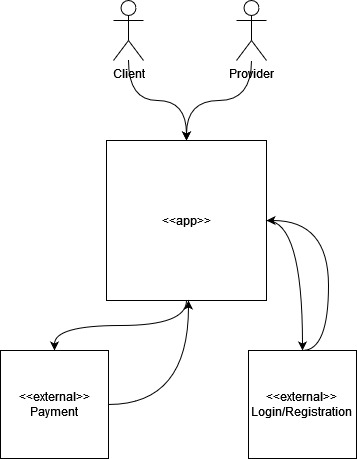
\includegraphics[width=0.7\textwidth]{assets/business_context.jpg}
    \caption{Preliminary functions}
    \label{fig:preliminary_use_case}
\end{figure}

\begin{table}[H]
    \setstretch{1.0}
    \begin{tabularx}{\textwidth}{lX}
    \toprule
    ID & Description   \\
    \midrule
    \gls{client} & Searches for a last time offer from a restaurant, bakery or pastry. \\
    \gls{provider} & Offers a still consumable product that was not sold during normal working time. \\
    Payment & Deals with the payment processing using registered information from another payment platforms. \\
    Login/Registration & Authenticated \gls{users} using logins from other platforms.  \\
    \bottomrule
    \end{tabularx}
\end{table}

\subsection{Technical Context}

\begin{table}[H]
    \setstretch{1.0}
    \begin{tabularx}{\textwidth}{lX}
    \toprule
    ID & Description   \\
    \midrule
    \gls{client} & AAAAAAAAAAAAAAAAAAAAAAAA \\
    \gls{provider} & AAAAAAAAAAAAAAAAAAAAAAAAAA \\
    Payment & AAAAAAAAAAAAAAAAA \\
    Login/Registration & AAAAAAAAAAAA  \\
    \bottomrule
    \end{tabularx}
\end{table}
    %\section{Solution and Strategy}
    %\section{Building Block View}

In this section we will describe the \gls{app} using some elements of the 4+1 Architectural View Model. With this model we will represent
the \gls{app} using five different views, which should focus on specific elements of the project. Each view provide
a different purpose \cite{refart:KR41}. For this project we will provide the 3 following views of the 4+1 Architectural View 
Model:

\begin{itemize}
    \item \textbf{Scenario view}: simple description for the end user 
    \item \textbf{Behaviour view}: description of the existing processes
    \item \textbf{Structural view}: object-oriented decomposition
\end{itemize}

The scenario view was presented in the figure \ref{fig:preliminary_use_case} of this project.

\subsection{Behaviour view}
The following \gls{activity diagram} depicts the register and login procedure within the app.

\begin{figure}[H]
    \centering
    \includegraphics[width=1\textwidth]{assets/login_AC.jpg}
    \caption{Login procedures}
    \label{fig:login_register}
\end{figure}


From the third party applications we expect the following interaction:

%% sequence diagram for login and payment



\subsection{Structural view}
To describe this view we choose a \gls{class diagram}. With it we may provide a static description of elements
of our app. This will be very relevant for the developing process of the \gls{app}.

The first part of the this diagram describes the element within the \gls{provider}. It contains one or more addresses and it 
can offer one or more products. A provider will also fall into the category restaurant, bakery or pastry.

\begin{figure}[H]
    \centering
    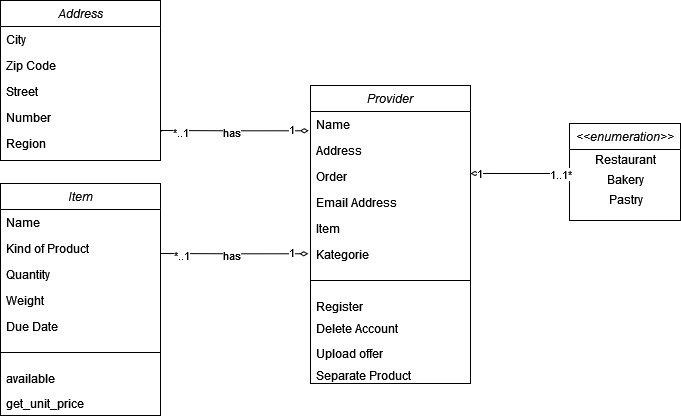
\includegraphics[width=0.8\textwidth]{assets/Provider_Addr_Item.jpg}
    \caption{Provider overview}
    \label{fig:Provider_addr_item}
\end{figure}
 
The class dedicated to the \glsplural{client} should be as simple as possible. It should provide basic interaction like
registering, logging, deleting account, viewing product and placing order. The two last actions will stablish the communication 
with the \glsplural{provider}.

\begin{figure}[H]
    \centering
    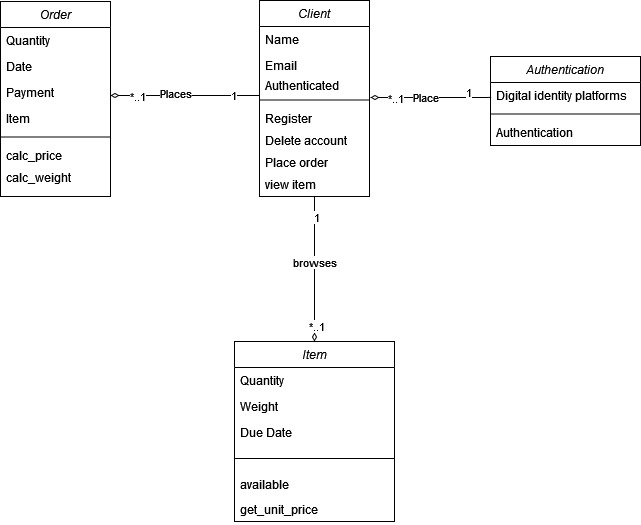
\includegraphics[width=0.8\textwidth]{assets/client_CD.jpg}
    \caption{Client Overview}
    \label{fig:client_CD}
\end{figure}

Finally we have an order placed by a \gls{client} and processed by a \gls{provider}. Here we will rely on a third party 
to stablish the payment procedures.

\begin{figure}[H]
    \centering
    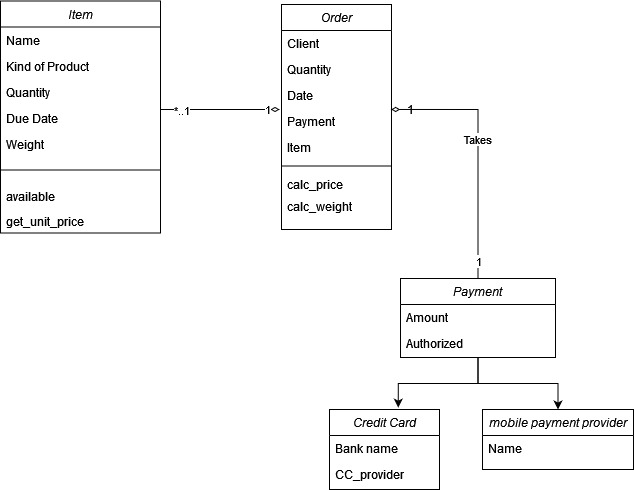
\includegraphics[width=0.7\textwidth]{assets/order_cd.jpg}
    \caption{Order Overview}
    \label{fig:order_cd}
\end{figure}

This final graphic show the whole classes in combination:

\begin{figure}[H]
    \centering
    \includegraphics[width=1\textwidth]{assets/classes_CD.jpg}
    \caption{Classes Overview}
    \label{fig:class_CD}
\end{figure}

 

    %\section{Runtime View}
    %\section{Deployment View}
    %\section{Crosscutting Concept} \label{Patterns_Tacticts}

In this chapter we will present the technical solutions that we will use to develop this project.
For each quality attribute we will present the chosen tactics.

\subsection{Solution for Usability}

The core of our app is how easy it is to use. We want our user to navigate through it without being overwhelmed with information
not related to the main objective: purchase a product or upload a product.

% \begin{table}[H]
%     \setstretch{1.0}
%     \begin{tabularx}{\textwidth}{|c|c|X|c|}
%         \toprule
%         \multicolumn{1}{c}{Tactict} & \multicolumn{1}{c}{Pattern} & \multicolumn{1}{c}{Motivation} & \multicolumn{1}{c}{QA} \\
%         \midrule
%         \textbf{Support User Initiative } & Observer & The interaction of the users is a main factor of our app.
%         We want them to have fully control of their actions either by cancelling or by resuming an action. & QA-1 \\
%         \textbf{Support User Initiative } & Lazy Registration & Avoid having to memorize another password and username
%         may increase the acceptance of the user. With this pattern we allow them also to browse in the app and seeing
%         what is available without being registered \cite{refonline:IDUI}. This may give a glimpse of what they get
%         if they join us. & QA-1 \\
%         \textbf{Support System Initiative} & Observer & By each upload from the \glsplural{provider} we want our
%         \glsplural{client} to have it on his device, without having to "ask" for it. & QA-1  \\
%         \bottomrule
%     \end{tabularx}
% \end{table}

To guarantee that our \glsplural{client} could get an easy and fast update from the \glsplural{provider} we choose 
the \textit{observer} pattern over the wellknown \glsfirst{MVC}. The former allow us to have focus on the implementation
on the different sides of our app, provider and clients. The latter has an inherent development burden for simple user
interfaces. Using \gls{MVC} for this first prototype would increase the difficult level and the time needed to provide a 
functional. 

Below there is a simple depict of this pattern:

\begin{figure}[H]
    \centering
    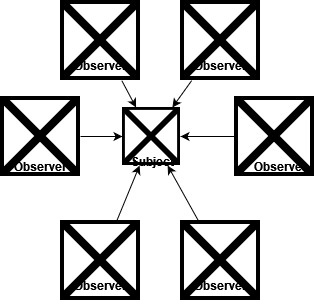
\includegraphics[width=1\textwidth]{assets/observer.jpg}
    \caption{Observer Pattern}
    \label{fig:simple_observer}
\end{figure}

The next diagram shows a more detailed version of the of the \textit{observer} pattern. This view intends to assist the development
team with the implementation of this pattern.

\begin{figure}[H]
    \centering
    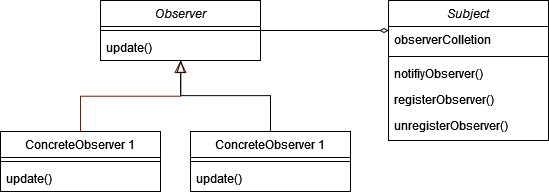
\includegraphics[width=1\textwidth]{assets/class_observer.jpg}
    \caption{Observer Pattern}
    \label{fig:class_observer}
\end{figure}

\begin{table}[H]
    \setstretch{1.0}
    \begin{tabularx}{\textwidth}{|c|c|X|c|}
    \toprule
    \multicolumn{1}{c}{Tactict} & \multicolumn{1}{c}{Pattern} & \multicolumn{1}{c}{Motivation} & \multicolumn{1}{c}{QA} \\
    \midrule
    \multicolumn{1}{|c|}{\multirow{2}{*}{Support User Initiative}} & Observer & The interaction of the users is a main factor
    of our app. We want them to have fully control of their actions either by cancelling or by resuming an action. The updates
    by the provider should be directly sent to the clients in a simple fast fashion.
    & \multirow{3}{*}{QA-1} \\
    \multicolumn{1}{|c|}{} & Lazy Registration & Avoid having to memorize another password and username may increase 
    the acceptance of the user. With this pattern we allow them also to browse in the app and seeing what is available 
    without being registered \cite{refonline:IDUI}. This may give a glimpse of what they get if they join us. The alternative
    is to have the user first register his credentials and then browser in the app. This burden would only make the get-to-know
    process slow and difficult. &  \\
    Support System Initiative & Observer & By each upload from the \glsplural{provider} we want our \glsplural{client} 
    to have it on his device, without having to "ask" for it.  &  \\ 
    \bottomrule
    \end{tabularx}
\end{table}




\subsection{Solution for Interoperability}

The communication with the third party components should during the whole lifetime of the App reliable. Since we are dealing 
with two different services, \gls{mobile payment gateway} and \gls{federated login}, we will describe the integration processes 
according to each specification.



\subsubsection{Payment Gateway}

The usage of \gls{mobile payment gateway} offers three possibilities \cite{refonline:ZOPG}:

\begin{itemize}
    \item Redirection to payment processor's page
    \item Payment data and processing inside the application
    \item Payment data entered in the app, but processed with an \gls{API}
\end{itemize}

The third option stays in direct contact with our top quality attribute, usability. Since we want to offer a easy shopping
experience, the payment process should also be harmonic with other features.

\begin{table}[H]
    \setstretch{1.0}
    \begin{tabularx}{\textwidth}{|c|c|X|c|}
        \toprule
        \multicolumn{1}{c}{Tactict} & \multicolumn{1}{c}{Pattern} & \multicolumn{1}{c}{Motivation} & \multicolumn{1}{c}{QA} \\
        \midrule
        \textbf{Limit Dependencies} & \Gls{wrapper} & The \gls{API} will be the intermediary for the payment process. For the 
        \glsplural{client} all visible steps will occur in the app, without being sent to another page. On the background
        the \gls{API} will receive the input and send it to the payment gateway. The verification takes place in gateway, 
        which then communicate with the financial institute of the client and send the payment to the \gls{provider} 
        \cite{refonline:ZOPG}. & QA-2 \\
        \bottomrule
    \end{tabularx}
\end{table}

\subsubsection{Federated Authentication}

Using of \gls{federated login} reduces burden of saving user credentials locally. It also improves the Usability so users
do not have to create and remember another username and password. The authentication process takes place on the third 
party operator, as seen in the picture \ref{fig:sequence_login_payment}. 

\begin{table}[H]
    \setstretch{1.0}
    \begin{tabularx}{\textwidth}{|c|c|X|c|}
        \toprule
        \multicolumn{1}{c}{Tactict} & \multicolumn{1}{c}{Pattern} & \multicolumn{1}{c}{Motivation} \\
        \midrule
        \textbf{\gls{microservice}} & \gls{API Gateway} & Increase of security, so the microservice is not directly
        exposed to the external world. It reduces the complexity of the microservice, since the gateway will have to deal
        with data transfer rate, tokens and other activities. Dealing with failures would also be handled and logged
        by the microservice \cite{refonline:javtop}. & QA-2\\
        \bottomrule
    \end{tabularx}
\end{table}

\subsection{Solution for Performance}

% remove this part, since it will not be firstly used

We want our app to have a fast (no more than 1 second) response time. By clicking on an offer a \gls{client} should
have it immediately displayed on his screen. Updated made by \glsplural{provider} should also be promptly available
for \glsplural{client} to browse.

\begin{table}[H]
    \setstretch{1.0}
    \begin{tabularx}{\textwidth}{|c|c|X|c|}
        \toprule
        \multicolumn{1}{c}{Tactics} & \multicolumn{1}{c}{Pattern} & \multicolumn{1}{c}{Motivation} & \multicolumn{1}{c}{QA} \\
        \midrule
        \textbf{Increase Resources} & \gls{Load Balancer} & This maybe implemented if, during the first test phase, we see that
        the usage of the app is so high that the existing components become overwhelmed. Specially during peak times we want our 
        users to have a smoothly and fast interaction with the app. \Glsplural{provider} and \glsplural{client} should perform their
        tasks, either browsing, purchasing or uploading offering without having to wait to get a response. With this
        decision all requests would be forwarded to the server that are available avoiding queuing of requests. & QA-3 \\
        \bottomrule
    \end{tabularx}
\end{table}

\newpage

\subsection{Solution for Security}

There are two security concerns that need to be addressed to the users. The first one deals with the authentication
and payment process. This will be managed by the third party providers. The second one involves the interaction of
the \glsplural{provider} with the app. Since this stakeholder can upload data and file to the app it is important
that only approved data type is inserted. In the table below we will describe the tactics used for the these
two concerns.

\begin{table}[H]
    \setstretch{1.0}
    \begin{tabularx}{\textwidth}{|c|c|X|c|}
        \toprule
        \multicolumn{1}{c}{Tactic} & \multicolumn{1}{c}{Pattern} & \multicolumn{1}{c}{Motivation} & \multicolumn{1}{c}{QA}\\
        \midrule
        \textbf{Validate Input} & \gls{Intercepting Validator} & \glsplural{provider} has a big interaction with the app.
        They can upload files and texts. To make sure that only secure element a inserted into the app, it is important
        that every input is analyzed before reaching the app and the \glsplural{client} \cite{refbook:CSWT}. & \multirow{3}{*}{QA-4} \\
        \shortstack{\textbf{Authenticate Actors} \\ \textbf{Authorize Actors}} & \shortstack{Authentication enforcer\\
        Authorization enforcer} & To avoid the connection of \gls{bots} we want to allow only registered users to interact with the functionalities 
        of the app. This will be done with the third party operators [\cite{refonline:wksp}]. & QA-4\\
        \bottomrule
    \end{tabularx}
\end{table}

% \begin{table}[H]
%     \setstretch{1.0}
%     \begin{tabularx}{\textwidth}{|c|c|X|c|}
%     \toprule
%     \multicolumn{1}{c}{Tactict} & \multicolumn{1}{c}{Pattern} & \multicolumn{1}{c}{Motivation} & \multicolumn{1}{c}{QA} \\
%     \midrule
%     \multicolumn{1}{|c|}{\multirow{2}{*}{Support User Initiative}} & Observer & The interaction of the users is a main factor
%     of our app. We want them to have fully control of their actions either by cancelling or by resuming an action.
%     & \multirow{3}{*}{QA-4} \\
%     \multicolumn{1}{|c|}{} & Lazy Registration & Avoid having to memorize another password and username may increase 
%     the acceptance of the user. With this pattern we allow them also to browse in the app and seeing what is available 
%     without being registered \cite{refonline:IDUI}. This may give a glimpse of what they get if they join us. &   \\

%     Support System Initiative & Observer & By each upload from the \glsplural{provider} we want our \glsplural{client} 
%     to have it on his device, without having to "ask" for it.  &  \\ 
%     \bottomrule
%     \end{tabularx}
% \end{table}

    %\section{Architectural Decisions Records}

In this section we will present the motivation to our decisions within this project.

\subsection{Chosen Preliminary Functionality}

\subsection{Highlighted Constraints}

\subsection{Stakeholders}

\subsection{Stakeholders}

\subsection{Stakeholders}

\begin{table}[H]
    \setstretch{1.0}
    \begin{tabularx}{\textwidth}{lX}
    \toprule
    ID & Reasoning   \\
    \midrule
    F-1 & Owner of a restaurant, bakery or pastry. \\
    F-2 & Person who wants to buy last minute products from a provider. \\
    F-3 & Team in charge of creating the application using existing tactics and creating new solutions. \\
    F-5 & ``Clean Up the Word (R)'' & Members of the  \\
    F-7 & Part of the society who aims to find environmental solutions to daily problems. \\
    F-8 & Part of the society who aims to find environmental solutions to daily problems. \\
    \bottomrule
    \end{tabularx}
\end{table}

include

describe each decision:
why this tactic/pattern
    \section{Quality Requirements}

\subsection{Quality Tree}

The priority of each element will be expressed using the following notation:

\begin{itemize}
    \item ([Customer view], [Architect view])
    \item H - High
    \item M - Medium
    \item L - Low
\end{itemize}

\Glsplural{user} and the development team have different perspective of an app. The former think about how attractive and easy to use
it is, the latter want to build something what achieves a goal. For that reason is the interpretation of the priority sometimes
so different, according to which group has been asked.

\begin{figure}[H]
    \centering
    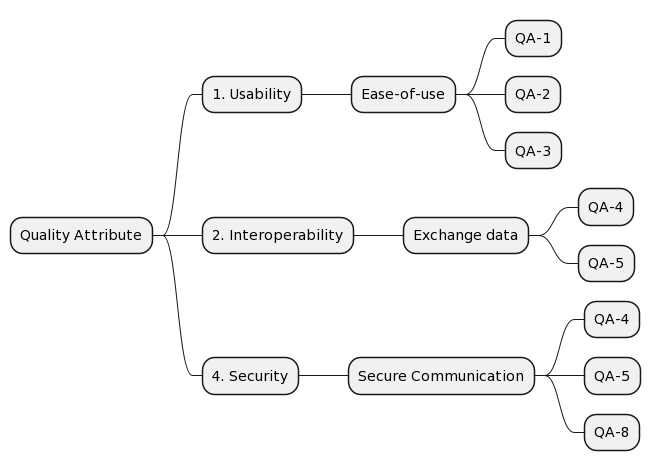
\includegraphics[width=0.7\textwidth]{assets/quality_tree.png}
    %\caption{Quality Tree}
    \label{fig:quality_tree}
\end{figure}

The next table presents the reason for the previous categorization regarding the priority of each quality attribute.

\begin{table}[H]
    \setstretch{1.0}
    \begin{tabularx}{\textwidth}{lXX}
        \toprule
        ID & Reasoning for \Glsplural{user} & Reasoning for Development Team  \\
        \midrule
        QA-1 & All important information should be there so his shop can be well promoted & 
        An initial registration with filter for the input is important, but aesthetically details are
        the goal now. \\
        QA-2 & Once he get something new, he wants to make it available & First we need to guarantee that no overrides occur
        than they see if it is promptly displayed. \\
        QA-3 & They want to browse and see all available options & Search engine can be very helpful, 
        but filtering can wait a litte, since it does not affect the app itself \\
        QA-4 & The most important is that they can use and purchase & This integration must be done fast and careful
        so no mistakes shows up. \\
        QA-5 & They just want to easily and secure pay, it does not matter how it works & The compliance with payment regulations is a must, since any mistake can costs huge fines
        and damage to the image of the company. \\
        QA-6 & They don't want to wast time with loading pages & The loading time can be fixed once there is a structure that allows
        loading in the first place.  \\
        QA-7 & They want to get confirmation that everything worked fine. & The communication between the \gls{API} and the payment provider show comply with all existing regulations. 
        Push notification can be added once the main feature works. \\
        QA-8 & That is something that they don't want to see, but want to make sure that it exists & Since the payment is processed by the third party operator, all concerns should be addressed to them
        and specified in the \glsfirst{SLA} \\
        \bottomrule
    \end{tabularx}
\end{table}


\subsection{Evaluation Scenarios} 
From the requirements, \ref{Requirement_Overview}, we could develop the following uses cases and depict the main quality 
attributes of this project. 

\begin{table}[H]
    \setstretch{1.0}
    \begin{tabularx}{\textwidth}{lX}
    \toprule
    Use Case & Description  \\
    \midrule
    UC-1: Register as \gls{client} & The \gls{client} registers an e-mail address.\\
    UC-2: Login & The \gls{client} logins in to the system. \\
    UC-3: Places an order & The \gls{client} chooses a \gls{provider}. \\
    UC-4: Register payment & The \gls{client} registers a payment method. \\
    UC-5: Register as \gls{provider} & The \gls{provider} registers their facility and products. \\
    UC-6: Update availability & The \gls{provider} uploads their product catalog. \\
    \bottomrule
    \end{tabularx}
    \label{table_use_case}
\end{table}

With the following use cases we will  be able to define the major quality attributes that are involved in the 
development of this application. They should be measurable and testable so we can verify if the system meets 
the needs our \glsplural{stakeholder} [\cite{refbook:DSHC}].

\begin{table}[H]
    \setstretch{1.0}
    \begin{tabularx}{\textwidth}{lcXc}
        \toprule
        ID & Quality Attribute & Scenario & Associated Use Case  \\
        \midrule
        QA-1 & Usability & A \gls{provider} is able to register his company, to specify the kind of products he offers 
        and upload a logo or picture of his shop and products in a easy and fast (within 5 Minutes) fashion. & UC-5 \\
        QA-2 & Usability & A \gls{provider} is able to update the offers at any time. &  UC-6 \\
        QA-3 & Usability & A \gls{client} is able to search and filter options. &  UC-6 \\
        QA-4 & Interoperability & A \gls{client} can register his e-mail using another account (Google, Microsoft, Facebook)
        in a \gls{federated login} & UC-1 \\
        QA-5 & Interoperability & A \gls{client} can pay the order using a \gls{mobile payment gateway} (e.g. Stripe, Square, PayPay, 
        SecurePay) & UC-4 \\
        %QA-5 & Performance & A \gls{client} registers his/her e-mail address and can immediately browse in the app. & UC-1 \\
        %QA-6 & Performance & A \gls{client} opens the app and he can immediately search for products or \glsplural{provider}. & UC-2 \\
        %QA-7 & Performance & A \gls{client} chooses a \gls{provider} and places his order. After the confirmation
        %of payment, a push-message is displayed in the app confirming the purchase. & UC-3 \\
        QA-8 & Security & The payment process should be secure and within the app. It should also give the \gls{client} the feeling
        of security. The \gls{client} inserts his payment information it is processed by the payment operator. & UC-4 \& QA-5 \\
        \bottomrule
    \end{tabularx}
\end{table}

\newpage
The defined quality attributes are represented in the following scenarios:

% add column id to the scenario

\begin{table}[H]
    \setstretch{1.0}
    \begin{tabularx}{\textwidth}{|c|X|X|X|}
        \hline
        \multicolumn{4}{c}{\textbf{Usability}} \\
        \hline
        \toprule
        \multicolumn{1}{|c|}{\textbf{Scenario}} & \multicolumn{3}{|c|}{\textbf{Value}} \\
        \midrule
        \multicolumn{1}{|c|}{ID} & \multicolumn{1}{|c|}{QS-1} & \multicolumn{1}{|c|}{QS-2} & \multicolumn{1}{|c|}{QS-3}  \\
        \hline
        Source & \Gls{provider} & Registered \Gls{provider} & \Gls{client}  \\
        \hline
        Stimulus & wants to register his shops & wants to make a last minute offer & wants to search/filter offers \\
        \hline
        Artifact & app & app & app \\
        \hline
        Environment & working time, during afternoon & peak period, between 4 and 7 pm on Friday & peak period, between 4 and 7 pm on Friday \\
        \hline
        Response & offer available in the app & immediate availability of the offer in the app & display of the filter/search output \\
        \hline
        Response Measure & How long did the registration and upload process take? How many and what kind of error messages did the \gls{provider} get?
        & How long did it take to upload an offer? How many and what kind of error messages did the \gls{provider} get? 
        & What kind of inputs did the user has to place until he finds what he wants? Did he have to type anything or were filter/search
        options available? How long it takes until the client finds a product? \\
        \bottomrule
    \end{tabularx}
\end{table}


% \begin{table}[H]
%     \begin{tabularx}{\textwidth}{|c|X|}
%         \hline
%         \multicolumn{2}{c}{\textbf{Usability - BACKUP}} \\
%         \hline
%         \toprule
%         \multicolumn{1}{c}{Scenario} & \multicolumn{1}{c}{Value} \\
%            \multicolumn{1}{|c|}{ID} & \multicolumn{1}{|c|}{QS-1} & \multicolumn{1}{|c|}{QS-2} & \multicolumn{1}{|c|}{QS-3}  \\
%            \hline
%         Source & \gls{provider} \\
%         Stimulus & wants to register his shops \\
%         Artifact & app \\
%         Environment & working time, during afternoon \\
%         Response & offer available in the app \\
%         Response Measure & How long did the registration and upload process take? How many and what kind of error messages
%         did the \gls{provider} get?\\
%          & \\
%         Source & Registered \gls{provider} \\
%         Stimulus & wants wants to make a last minute offer \\
%         Artifact & app \\
%         Environment & peak period, between 4 and 7 pm on Friday \\
%         Response & immediate availability of the offer in the app \\
%         Response Measure & How long did it take to upload an offer? How many and what kind of error messages did the 
%         \gls{provider} get? \\
%         & \\
%         Source & Registered \gls{client} \\
%         Stimulus & wants to search/filter offers \\
%         Artifact & app \\
%         Environment & peak period, between 4 and 7 pm on Friday \\
%         Response & display of the filter/search output \\
%         Response Measure & What kind of inputs did the user has to place until he finds what he wants?
%         Did he have to type anything or were filter/search options available? How long it takes until the client
%         finds a product? \\
%         \bottomrule
%     \end{tabularx}
% \end{table}

 \begin{table}[H]
    \setstretch{1.0}
    \begin{tabularx}{\textwidth}{|c|X|X|}
        \hline
        \multicolumn{3}{c}{\textbf{Interoperability}} \\
        \hline
        \toprule
        \multicolumn{1}{|c|}{\textbf{Scenario}} & \multicolumn{2}{|c|}{\textbf{Value}} \\
        \midrule
        \multicolumn{1}{|c|}{ID} & \multicolumn{1}{|c|}{QS-4} & \multicolumn{1}{|c|}{QS-5}  \\
        \hline
        Source & \Gls{client} & \Gls{client}  \\
        \hline
        Stimulus & wants register using a \gls{federated login} & wants to pay using existing mobile payment account \\
        \hline
        Artifact & app and \gls{federated login} provider & app and \gls{mobile payment gateway} \\
        \hline
        Environment & peak period (on the context of the \gls{federated login} provider) & peak period (on the context of the gateway) \\
        \hline
        Response & authentication succeed or failed & confirmation / declined \\
        \hline
        Response Measure & How much data was transmitted and how much was queued? Focus on System overload [\cite{refart:MKMS}]
        & Total amount generated data in the app that are transferred and processed and rejected by the gateway? Focus o connectivity 
        and system overload [\cite{refart:MKMS}] \\
        \bottomrule
    \end{tabularx}
\end{table}

% \begin{table}[H]
%     \begin{tabularx}{\textwidth}{|c|X|}
%         \hline
%         \multicolumn{2}{c}{\textbf{Interoperability - Backup}} \\
%         \hline
%         \toprule
%         \multicolumn{1}{c}{Scenario} & \multicolumn{1}{c}{Value} \\
%         \midrule
%         Source & \gls{client} \\
%         Stimulus & wants register using a \gls{federated login} \\
%         Artifact & app and \gls{federated login} provider  \\
%         Environment & peak period (on the context of the \gls{federated login} provider)\\
%         Response & authentication succeed or failed\\
%         Response Measure & How much data was transmitted and how much was queued? \\
%         Focus & System overload \cite{refart:MKMS} \\
%         & \\
%         Source & \gls{client} \\
%         Stimulus & wants to pay using existing mobile payment account \\
%         Artifact & app and \gls{mobile payment gateway}  \\
%         Environment & peak period (on the context of the gateway)\\
%         Response & confirmation / declined \\
%         Response Measure & Total amount generated data in the app that are transferred and processed and rejected
%         by the gateway \\
%         Focus & Connectivity and System overload \cite{refart:MKMS} \\
%         \bottomrule
%     \end{tabularx}
% \end{table}

% \begin{table}[H]
%     \setstretch{1.0}
%     \begin{tabularx}{\textwidth}{|c|X|X|X|}
%         \hline
%         \multicolumn{4}{c}{\textbf{Performance}} \\
%         \hline
%         \toprule
%         \multicolumn{1}{|c|}{\textbf{Scenario}} & \multicolumn{3}{|c|}{\textbf{Value}} \\
%         \midrule
%         \multicolumn{1}{|c|}{ID} & \multicolumn{1}{|c|}{QS-6} & \multicolumn{1}{|c|}{QS-7} \\
%         \hline
%         Source & \Gls{client} & \Gls{client} & \Gls{client}  \\
%         \hline
%         Stimulus & wishes to create an account & wants to search for a \gls{provider} & places an order \\
%         \hline
%         Artifact & app & app & app \\
%         \hline
%         Environment & weekend between 3 and 7 PM & peak period, between 6 and 7 pm on a Friday & peak period, between 6 and 7 pm on a Friday \\
%         \hline
%         Response & immediate access to the app  & immediate access to the offers  & confirmation of payment / payment declined \\
%         \hline
%         Response Measure & time between confirmation and access & how quickly does the client's device get update of availabilities 
%         & How long did take until the client get the confirmation/declined of payment? \\
%         \bottomrule
%     \end{tabularx}
% \end{table}


% \begin{table}[H]
%     \begin{tabularx}{\textwidth}{|c|X|}
%         \hline
%         \multicolumn{2}{c}{\textbf{Performance - Backup}} \\
%         \hline
%         \toprule
%         \multicolumn{1}{c}{Scenario} & \multicolumn{1}{c}{Value} \\
%         \midrule
%         Source & \gls{client}  \\
%         Stimulus & wishes to create an account \\
%         Artifact & app \\
%         Environment & weekend between 3 and 7 PM \\
%         Response & immediate access to the app \\
%         Response Measure & time between confirmation and access \\
%          & \\
%         Source & \gls{client}  \\
%         Stimulus & wants to search for a \gls{provider} \\
%         Artifact & app \\
%         Environment & peak period, between 6 and 7 pm on a Friday \\
%         Response & immediate access to the offers \\
%         Response Measure & how quickly does the client's device get update of availabilities \\
%         & \\
%         Source & \gls{client}  \\
%         Stimulus & places an order \\
%         Artifact & platform \\
%         Environment & peak period, between 6 and 7 pm on a Friday \\
%         Response & confirmation of payment / payment declined \\
%         Response Measure & How long did take until the client get the confirmation/declined of payment?\\
%         \bottomrule
%     \end{tabularx}
% \end{table}

\begin{table}[H]
    \setstretch{1.0}
    \begin{tabularx}{\textwidth}{|c|X|X|}
        \hline
        \multicolumn{3}{c}{\textbf{Security}} \\
        \hline
        \toprule
        \multicolumn{1}{|c|}{\textbf{Scenario}} & \multicolumn{2}{|c|}{\textbf{Value}} \\
        \midrule
        \multicolumn{1}{|c|}{ID} & \multicolumn{1}{|c|}{QS-6} & \multicolumn{1}{|c|}{QS-7}  \\
        \hline
        Source & \Gls{client} & \Gls{client} \\
        \hline
        Stimulus & clicks on registration using an existing login & click on pay using an existing mobile payment account \\
        \hline
        Artifact & app, \gls{API Gateway} and \gls{federated login} provider & app, \gls{microservice} and \gls{mobile payment gateway} \\
        \hline
        Environment & peak period (on the context of the \gls{federated login} provider) & peak period (on the context of the gateway) \\
        \hline
        Response & authentication succeed or failed & confirmation / declined \\
        \hline
        Response Measure & Required time and effort to intercept and/or block requests (create \glsfirst{DoS})
        & Extension and impact to image/damage of the app/company in case of attack \\
        \bottomrule
    \end{tabularx}
\end{table}
    %\section{Risk and Technical Debt}

To measure the risks of this project we will use the following 3x3 risk matrix, which will help us develop the 
\gls{risk assessment}:

\begin{figure}[H]
    \centering
    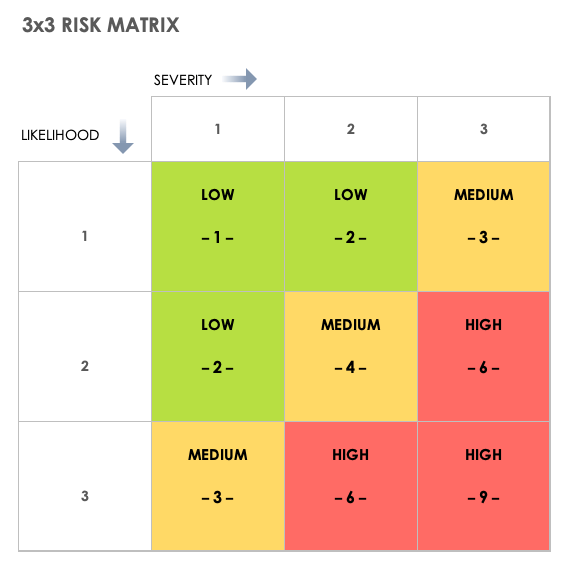
\includegraphics[width=0.5\textwidth]{assets/Risk-Matrix.png}
    \caption{3x3 Risk Matrix Template\\ Source: \citet{refonline:smtrisk}  }
    \label{fig:risk_matrix_template}
\end{figure}


The elements used to identify the risk are shown in the picture below:

\begin{figure}[H]
    \centering
    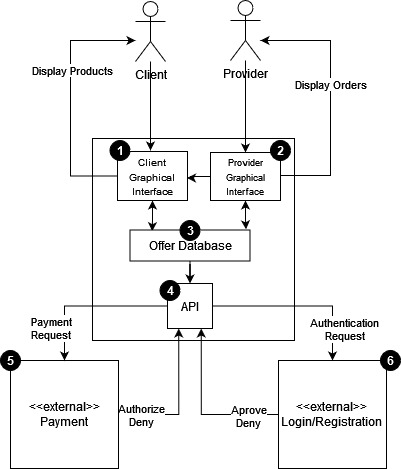
\includegraphics[width=0.4\textwidth]{assets/risk_technical_context.jpg}
    \caption{Modified from Figure \ref{fig:technical_context}}
    \label{fig:risk_technical_context}
\end{figure}

\newpage
The following risk table was defined after several discussion with the team members:

% backup
% \begin{table}[H]
%     \centering
%     \resizebox{\textwidth}{!}{%
%     \begin{tabular}{|l|llllll}
%     \toprule
%     \multicolumn{1}{c}{\textbf{Risk Criteria}}              & \multicolumn{6}{c}{\textbf{Element ID}} \\ \hline
%     \midrule
%     \multicolumn{1}{c}{}              & \multicolumn{1}{c}{\textbf{1}} & \multicolumn{1}{c}{\textbf{2}} & \multicolumn{1}{c}{\textbf{3}} & \multicolumn{1}{c}{\textbf{4}} & \multicolumn{1}{c}{\textbf{5}} & \multicolumn{1}{c}{\textbf{6}} \\ \hline
%     \multicolumn{1}{|l|}{\textbf{Unproven technology}}      & \multicolumn{1}{l|}{1} & \multicolumn{1}{l|}{1} & \multicolumn{1}{l|}{1} & \multicolumn{1}{l|}{1} & \multicolumn{1}{l|}{1} & \multicolumn{1}{l|}{1} \\ \hline
%     \multicolumn{1}{|l|}{\textbf{Performance}}              & \multicolumn{1}{l|}{2} & \multicolumn{1}{l|}{2} & \multicolumn{1}{l|}{1} & \multicolumn{1}{l|}{1} & \multicolumn{1}{l|}{1} & \multicolumn{1}{l|}{1} \\ \hline
%     \multicolumn{1}{|l|}{\textbf{Scalability}}              & \multicolumn{1}{l|}{1} & \multicolumn{1}{l|}{1} & \multicolumn{1}{l|}{2} & \multicolumn{1}{l|}{1} & \multicolumn{1}{l|}{1} & \multicolumn{1}{l|}{1} \\ \hline
%     \multicolumn{1}{|l|}{\textbf{Availability}}             & \multicolumn{1}{l|}{1} & \multicolumn{1}{l|}{1} & \multicolumn{1}{l|}{4} & \multicolumn{1}{l|}{2} & \multicolumn{1}{l|}{1} & \multicolumn{1}{l|}{1} \\ \hline
%     \multicolumn{1}{|l|}{\textbf{Data loss}}                & \multicolumn{1}{l|}{1} & \multicolumn{1}{l|}{1} & \multicolumn{1}{l|}{3} & \multicolumn{1}{l|}{1} & \multicolumn{1}{l|}{1} & \multicolumn{1}{l|}{1} \\ \hline
%     \multicolumn{1}{|l|}{\textbf{Single points of failure}} & \multicolumn{1}{l|}{1} & \multicolumn{1}{l|}{1} & \multicolumn{1}{l|}{4} & \multicolumn{1}{l|}{4} & \multicolumn{1}{l|}{1} & \multicolumn{1}{l|}{1} \\ \hline
%     \multicolumn{1}{|l|}{\textbf{Security}}                 & \multicolumn{1}{l|}{1} & \multicolumn{1}{l|}{2} & \multicolumn{1}{l|}{3} & \multicolumn{1}{l|}{2} & \multicolumn{1}{l|}{2} & \multicolumn{1}{l|}{2} \\ \hline
%     \bottomrule
% \end{tabular}%
%     }
% \end{table}

\begin{table}[H]
    \centering
    \resizebox{\textwidth}{!}{%
    \begin{tabular}{|l|l|l|l|l|l|l|}
    \toprule
    \multicolumn{1}{c}{\multirow{2}{*}{\textbf{Risk Criteria}}} & \multicolumn{6}{c}{\textbf{Element ID}} \\ 
    %\midrule
    \multicolumn{1}{c}{}            & \multicolumn{1}{c}{\textbf{1}} & \multicolumn{1}{c}{\textbf{2}} & \multicolumn{1}{c}{\textbf{3}} & \multicolumn{1}{c}{\textbf{4}} & \multicolumn{1}{c}{\textbf{5}} & \multicolumn{1}{c}{\textbf{6}} \\ \hline
    \textbf{Unproven technology}      & 1 & 1 & 1 & 1 & 1 & 1 \\ \hline
    \textbf{Performance}              & 2 & 2 & 1 & 1 & 1 & 1 \\ \hline
    \textbf{Scalability}              & 1 & 1 & 2 & 1 & 1 & 1 \\ \hline
    \textbf{Availability}             & 1 & 1 & 4 & 2 & 1 & 1 \\ \hline
    \textbf{Data loss}                & 1 & 1 & 3 & 1 & 1 & 1 \\ \hline
    \textbf{Single points of failure} & 1 & 1 & 4 & 4 & 1 & 1 \\ \hline
    \textbf{Security}                 & 1 & 2 & 3 & 2 & 2 & 2 \\ \hline
    %\bottomrule
\end{tabular}%
    }
\end{table}




\subsection{Motivation}

\begin{table}[H]
    \setstretch{1.0}
        \begin{tabularx}{\textwidth}{|l|X|X|X|}
        \toprule
           \textbf{Risk Criteria} & \textbf{1 Client Graphical Interface} & \textbf{2 Provider Graphical Interface} & \textbf{3 Offer Database} \\
        \midrule
        \textbf{Unproven technology}& \textit{not applicable} & \textit{not applicable} & \textit{not applicable} \\
        \hline
        \textbf{Performance} & Concerns regarding a such dynamic shop. Data displayed & Concerns regarding a such dynamic shop. Data update. & \textit{not applicable} \\
        \hline
        \textbf{Scalability} & \textit{not applicable} & \textit{not applicable} & One database can be overwhelmed if the number of user is not limited for this prototype version. \\
        \hline
        \textbf{Availability} & \textit{not applicable} & \textit{not applicable} & In case of intense traffic the latency can be more than expected. \\
        \hline
        \textbf{Data loss} & \textit{not applicable} & \textit{not applicable} & Nowadays no company can survive in case of data loss. Technical damages can be 
        mostly easy fixed, but moral damage stays forever. \\
        \hline
        \textbf{Single points of failure} & \textit{not applicable} & \textit{not applicable} & Only one component gives always this risk. Increasing the 
        number of components increases also the total development costs \\
        \hline
        \textbf{Security} & \textit{not applicable} the client's input is always processed
        by the API and by the third party providers & If no strong data filtering exists, providers can upload
        malicious files or execute unwished commands. & The filtering of the input should occur mostly on the server side, Source
        no external access can figure out, how it is implemented. \\
        \bottomrule
    \end{tabularx}
\end{table}

\begin{table}[H]
    \setstretch{1.0}
    \begin{tabularx}{\textwidth}{|l|X|X|X|}
        \toprule
        \textbf{Risk Criteria} & \textbf{4 API} & \textbf{5 External Payment Service} & \textbf{6 External Authentication Service} \\
        \midrule
        \textbf{Unproven technology} & \textit{not applicable} & \textit{not applicable}  & \textit{not applicable}  \\
        \hline
        \textbf{Performance} & \textit{not applicable} & \textit{not applicable}  & \textit{not applicable} \\
        \hline
        \textbf{Scalability} & \textit{not applicable} & \textit{not applicable} & \textit{not applicable} \\
        \hline
        \textbf{Availability} & The access to the products become unstable. & \textit{not applicable} & \textit{not applicable} \\
        \hline
        \textbf{Data loss} & \textit{not applicable} & \textit{not applicable} & \textit{not applicable} \\
        \hline
        \textbf{Single points of failure} & In case of failure login, registration and payment are compromised. & \textit{not applicable} & \textit{not applicable} \\
        \hline
        \textbf{Security} & Lack of practical experience within the team about this topic. we rely on the service provided by the third party companies 
        & SLA Less than 99.5\% but equal to or greater than 95.0\% \cite{refmisc:paycSLA} & SLA < 99.99\% - >= 99.9\% \cite{refmisc:auth0sla}	\\
        \bottomrule
    \end{tabularx}
\end{table}
%1 - 
%
    %\include{12_Glossary}
    \nocite{*}
    \bibliography{reference}
    \bibliographystyle{apalike}
        
\end{document}